\documentclass{article}

\usepackage{graphicx}

\begin{document}

\title{Homework 1}
\author{Mitchel Fields}
\date{2/26/15}
\maketitle

\paragraph{1. FCFS}\mbox{}\\
Average turnaround: 369.95 seconds/job\\
Average wait time: 362.87 seconds\\
Throughput: 11.8 jobs/minute

\paragraph{2. RR}\mbox{}\\
Average turnaround: 336.38 seconds/job\\
Average wait time: 329.3 seconds\\
Throughput: 11.8 jobs/minute

\paragraph{3. SJF}\mbox{}\\
Average turnaround: 185.63 seconds/job\\
Average wait time: 178.55 seconds\\
Throughput: 11.8 jobs/minute\\\\
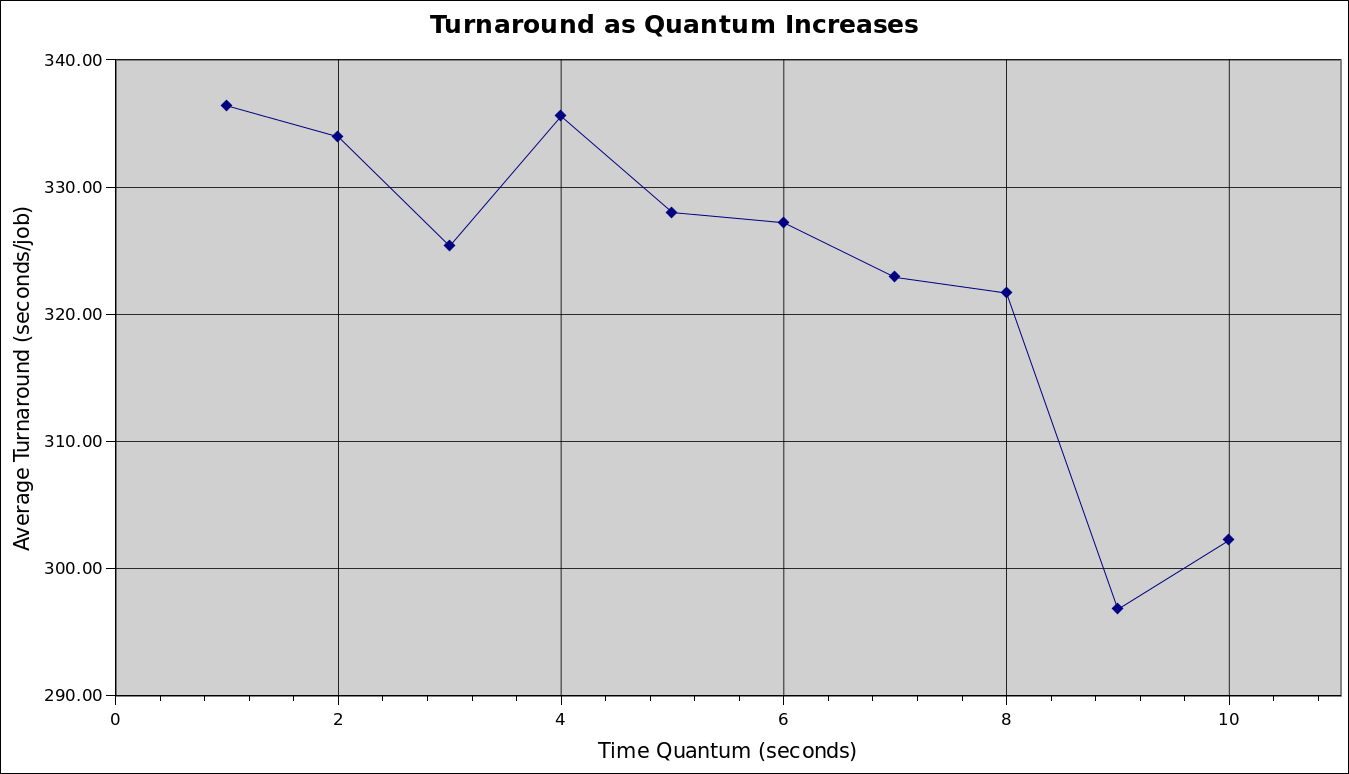
\includegraphics[width=\linewidth]{TurnaroundQuantum}\\\\
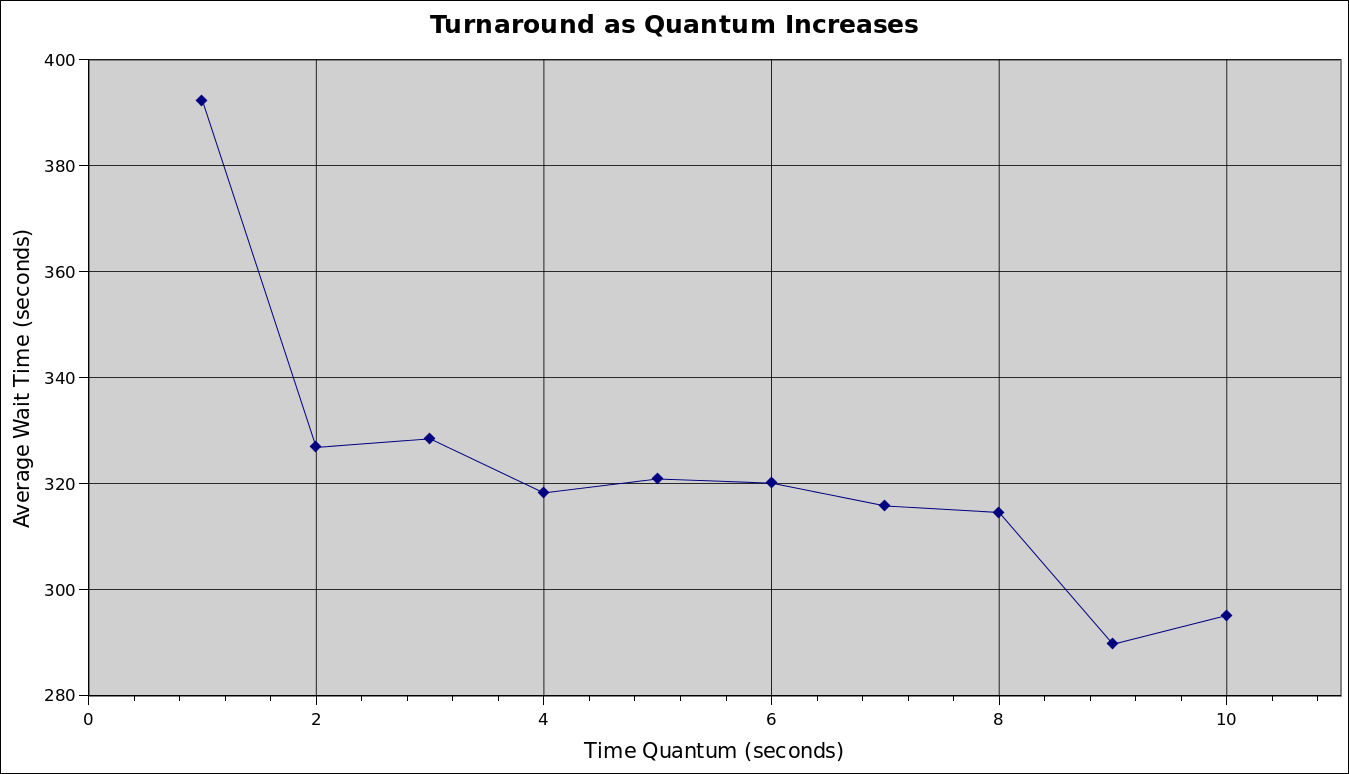
\includegraphics[width=\linewidth]{WaitTimeQuantum}

\paragraph{4.}\mbox{}\\
Shortest job first minimizes wait time as a result of the shortest jobs executing first. This minimizes the wait time of the following jobs as much as possible; the shortest jobs accrue the shortest wait time for the other, longer, jobs.

\end{document}